% 隔離テスト用ドライバ: 10-13 のみを単独ビルド（共有 main.tex には影響しない）
% 旧 _drv912 を 2026-06-07 の再構成（熱統合=4挿入で +1 ずれ）に合わせて更新。
\documentclass[11pt,aspectratio=43,dvipsnames]{beamer}
\usepackage{luatexja}
\usepackage[match]{luatexja-fontspec}
\setmainjfont{HaranoAjiGothic}
\setsansjfont{HaranoAjiGothic}
\renewcommand{\kanjifamilydefault}{\gtdefault}
\usepackage{amsmath, amssymb}
\usepackage[version=4]{mhchem}
\usepackage{booktabs}
\usepackage{multirow}
\usepackage{colortbl}
\usepackage{graphicx}
\graphicspath{{figures/}}
\usepackage{pgfplots}
\pgfplotsset{compat=1.18}
% =====================================================================
%  seminar テーマ定義（既存 Marp デザインの Beamer 再現）
%  ・濃青の恒常ヘッダーバー（セクション名＋ページ番号）
%  ・専用表紙（アクセントライン＋グラデ背景）
%  ・本文は白地・濃青見出し
%  main.tex から \input する（パッケージではなく生プリアンブル）
% =====================================================================

% ---- ベース：装飾の少ないテーマから組む -----------------------------
\usetheme{default}
\usefonttheme{professionalfonts}
\setbeamertemplate{navigation symbols}{}   % ナビゲーション記号を消す

% ---- TikZ（ヘッダー・表紙・矢印などで使用）-------------------------
\usepackage{tikz}
\usetikzlibrary{arrows.meta, positioning, calc, shapes.geometric, fit, patterns}

% ---- 配色（ルール準拠）---------------------------------------------
\definecolor{HeaderBlue}{HTML}{0f5a7a}   % ヘッダー・見出しの濃青
\definecolor{DateGray}{HTML}{334b5e}     % 表紙の日付グレー
\definecolor{TitleBG}{HTML}{edf5fb}      % 表紙グラデの薄青

% コンテンツ用パレット（図・ハイライト・矢印で共通利用）
\definecolor{ArrowBlue}{HTML}{1F6FC4}    % 矢印・強調の青
\definecolor{HiPink}{HTML}{F4B6BE}       % ハイライト見出し（暖色）
\definecolor{HiBlue}{HTML}{C7DCEF}       % ハイライト見出し（寒色）
\definecolor{IpaBlue}{HTML}{1F5FC4}      % グラフ系列1（青）
\definecolor{DipeOrange}{HTML}{E8821E}   % グラフ系列2（橙）
\definecolor{SpRed}{HTML}{C0392B}        % 反応式：プロピレン強調の赤
\definecolor{SpBlue}{HTML}{1F6FC4}       % 反応式：エテン・エタン・CH0.5 の青

% 帯（ヘッダーバー）のパート別配色（寒色グラデ）。本文枠線は HeaderBlue のまま。
%  1-4 導入・全体像／5-9 反応・反応器／10-13 分離／14-17 最適化・経済・結言
\definecolor{barA}{HTML}{0F5A7A}   % 1-4  青緑
\definecolor{barB}{HTML}{1D6E6E}   % 5-9  シアン寄り
\definecolor{barC}{HTML}{2E4C8A}   % 10-13 青
\definecolor{barD}{HTML}{4A3C84}   % 14-17 紫

\setbeamercolor{normal text}{fg=black, bg=white}
\setbeamercolor{frametitle}{fg=HeaderBlue, bg=white}
\setbeamercolor{itemize item}{fg=HeaderBlue}
\setbeamercolor{itemize subitem}{fg=HeaderBlue}
\setbeamercolor{block title}{fg=white, bg=HeaderBlue}
\setbeamercolor{block body}{fg=black, bg=TitleBG}
\setbeamercolor{alerted text}{fg=HeaderBlue}

% ---- フォントサイズ（Marp px をおおよそ pt に対応）------------------
\setbeamerfont{frametitle}{size=\large, series=\bfseries}   % スライド見出し ~44px

% ---- 恒常ヘッダーバー（headline）-----------------------------------
%  左：セクション名（無ければロゴ枠）／右：ページ番号
\newcommand{\HeaderLogo}{}   % ロゴを入れるなら \renewcommand で画像指定
% 本線の総枚数（分母）。appendix に入ると分子がこれを超え、本線/付録を見分けられる。
\newcommand{\MainTotal}{17}
% パート別に帯色を選ぶ：1-4=barA／5-9=barB／10-13=barC／14-17=barD。
% スライド4の独自帯（CC・GCC）など headline を上書きする箇所でも呼べるよう独立コマンド化。
% 併せて本文アクセント色 HeaderBlue 自体をそのパート色へ再定義し、各スライドの
% 図・枠線・矢印・ボックス（HeaderBlue 参照）をパート色に連動させる（\colorlet は大域的）。
% headline はフレーム本文より前に組まれるため、ここでの再定義が本文に効く。
\newcommand{\SetBarColor}{%
  \ifnum\insertframenumber<5\setbeamercolor{headerbar}{fg=white, bg=barA}\colorlet{HeaderBlue}{barA}%
  \else\ifnum\insertframenumber<10\setbeamercolor{headerbar}{fg=white, bg=barB}\colorlet{HeaderBlue}{barB}%
  \else\ifnum\insertframenumber<14\setbeamercolor{headerbar}{fg=white, bg=barC}\colorlet{HeaderBlue}{barC}%
  \else\setbeamercolor{headerbar}{fg=white, bg=barD}\colorlet{HeaderBlue}{barD}%
  \fi\fi\fi}
\setbeamertemplate{headline}{%
  \ifnum\insertframenumber>0\relax
    \SetBarColor
    \begin{beamercolorbox}[wd=\paperwidth, ht=4.5ex, dp=1.8ex,
                           leftskip=1.2em, rightskip=1.2em]{headerbar}%
      \color{white}\bfseries\large
      \insertsectionhead%
      \hfill
      \insertframenumber/\MainTotal%
    \end{beamercolorbox}%
  \fi
}
\setbeamercolor{headerbar}{fg=white, bg=barA}
\setbeamertemplate{footline}{}             % フッターは使わない
\setbeamersize{text margin left=3mm, text margin right=3mm}  % 本文を横幅ぎりぎりまで

% 【必須ルール】帯と本文の間の余白を詰める（全スライド共通）。
%  beamer 既定の天井スキップで本文が帯から離れるのを、headline 直後の負スキップで打ち消す。
%  情報量最優先：無駄な上余白は作らない。各スライドは [t] 推奨。
\addtobeamertemplate{headline}{}{\vskip-2.6ex}

% frametitle はバーの直下に置く（左寄せ・濃青・太字）
\setbeamertemplate{frametitle}{%
  \vskip0.6ex
  \hspace{0.6em}\usebeamerfont{frametitle}\usebeamercolor[fg]{frametitle}\insertframetitle\par
  \vskip0.2ex
}

% ---- 箇条書きをシンプルに ------------------------------------------
\setbeamertemplate{itemize item}{\textbullet}
\setbeamertemplate{itemize subitem}{--}

% =====================================================================
%  再利用ヘルパー（どのスライドでも使える共通部品）
% =====================================================================
% 青い矢印 →（行中に置ける。結論や対応関係の明示に）
\newcommand{\bluearrow}{\tikz[baseline=-0.5ex]\draw[ArrowBlue, line width=1pt,
  -{Stealth[length=2.2mm]}] (0,0)--(0.55,0);}

% ハイライト見出し  \hilite{色}{テキスト}  例: \hilite{HiPink}{IPA選択率の温度依存性}
\newcommand{\hilite}[2]{\colorbox{#1}{\bfseries\normalsize #2}}

% パラメータ表  \paramtable{ 項目 & 値 \\ ... }  （左:項目 右:値、単位は数式推奨）
\newcommand{\paramtable}[1]{%
  {\footnotesize\renewcommand{\arraystretch}{1.15}%
   \begin{tabular}{@{\hspace{1em}}ll@{}}#1\end{tabular}}}

% =====================================================================
%  専用表紙コマンド  \seminartitlepage
%  ルール準拠：アクセントライン(120x8px相当) + 160度グラデ背景
%               h1 60px / h2 34px濃青 / 著者27px / 日付22pxグレー
%  使い方: \title{} \subtitle{} \author{} \date{} を設定後に呼ぶ
% =====================================================================
\newcommand{\seminartitlepage}{%
  \begin{frame}[plain]
    \begin{tikzpicture}[remember picture, overlay]
      % 背景グラデ（左上 薄青 → 右下 白、斜め）
      \shade[top color=TitleBG, bottom color=white, shading angle=20]
        (current page.south west) rectangle (current page.north east);
      % アクセントライン（上から少し下げて左に）
      \fill[HeaderBlue]
        ([xshift=9mm, yshift=-12mm]current page.north west)
        rectangle ++(16mm, 1.1mm);
      % テキストブロック（左寄せ・縦中央付近）
      \node[anchor=center, text width=0.86\paperwidth, align=center]
            at (current page.center) {%
        {\fontsize{22pt}{28pt}\selectfont\bfseries\color{black}\inserttitle\par}
        \vspace{0.3em}
        {\fontsize{16pt}{20pt}\selectfont\bfseries\color{HeaderBlue}\insertsubtitle\par}
        \vspace{1.0em}
        {\fontsize{13pt}{17pt}\selectfont\color{black}\insertauthor\par}
        \vspace{0.4em}
        {\fontsize{11pt}{14pt}\selectfont\color{DateGray}\insertdate\par}
      };
    \end{tikzpicture}
  \end{frame}
}

\setlength{\overfullrule}{6pt}
\begin{document}
\setcounter{framenumber}{9}
\section{分離戦略}% =====================================================================
%  10  分離戦略 — 左=分離の考え方（タイトル付き説明＋沸点マップ）｜右=工程フロー＋膜有無比較
%  source_memo: trial #201・07章 Table7.1/Fig7.1。分離目標(要求純度)を主役に:
%   C3H6 99.5wt%(α≈1.07)・H2 99.9mol%。脱ブタン=C4除去、脱エタン=軽質分離。
%   膜有無比較(共通フィード C3H6 60.7mol%): 膜+塔 TAC135/117段/94m vs 塔単独 TAC1625/200段/156m。
%  方針：まず左で「沸点→分離操作」の考え方を示し、右で工程フローと膜の効果へ。
%        左右は全高の仕切りで分ける。重なり・はみ出し・無駄余白なし。丸括弧禁止。
% =====================================================================
\definecolor{SepGreen}{HTML}{2E9E5B}
\begin{frame}[t]

  \vspace{0.05em}

  \begin{columns}[T,onlytextwidth]
    % ===== 左：分離の考え方（タイトル付き説明＋沸点マップ）｜右端に全高の仕切り =====
    \begin{column}{0.34\textwidth}
      \resizebox{!}{\dimexpr\textheight-6mm\relax}{%
      \begin{tikzpicture}[
        x=1cm, y=1cm, >=Stealth, font=\small,
        cut/.style={dashed, HeaderBlue, line width=0.8pt, -{Stealth[length=2mm]}},
        cuthard/.style={dashed, SpRed, line width=1.1pt, -{Stealth[length=2.2mm]}},
        tick/.style={HeaderBlue, line width=0.8pt},
        lab/.style={anchor=west, font=\small\bfseries},
        cmp/.style={anchor=west, font=\small},
        val/.style={anchor=east, font=\footnotesize, text=black!55},
      ]
        \useasboundingbox (-0.7,-0.9) rectangle (4.55,10.7);
        % --- 全高の仕切り縦線（右端：右の工程と分ける）---
        \draw[black!35, line width=0.9pt] (4.35,-0.8) -- (4.35,10.6);
        % --- タイトル付き説明 ---
        \node[anchor=north west, font=\large\bfseries, text=HeaderBlue] at (-0.6,10.5) {分離の考え方};
        \node[anchor=north west, font=\normalsize, text width=4.6cm, align=left] at (-0.6,9.7)
          {成分を沸点順に並べ、各境界に分離操作を割り当てた。沸点差の大きい境界は蒸留、沸点差 $6$ K と小さい C3 対のみ膜＋蒸留で分離。};
        % --- 沸点マップ（軸＝上が高沸点）---
        \draw[HeaderBlue, line width=1.3pt, ->] (0.3,0.5) -- (0.3,7.15);
        \node[anchor=west, font=\footnotesize, text=black!60] at (0.5,6.98) {[$^\circ$C]};
        \foreach \y/\name/\bp in {6.7/{$\mathrm{C_4H_{10}}$}/{$-1$}, 3.9/{$\mathrm{C_2H_6}$}/{$-89$}, 2.6/{$\mathrm{CH_4}$}/{$-161$}, 1.0/{$\mathrm{H_2}$}/{$-253$}}{
          \draw[tick] (0.15,\y) -- (0.45,\y);
          \node[cmp] at (0.5,\y) {\name};
          \node[val] at (0.0,\y) {\bp};
        }
        % C3 ペア（赤・近接）
        \draw[tick, SpRed] (0.15,5.5) -- (0.45,5.5);
        \draw[tick, SpRed] (0.15,5.1) -- (0.45,5.1);
        \node[cmp, text=SpRed] at (0.5,5.5) {$\mathrm{C_3H_8}$};
        \node[cmp, text=SpRed] at (0.5,5.1) {$\mathrm{C_3H_6}$};
        \node[val, text=SpRed] at (0.0,5.5) {$-42$};
        \node[val, text=SpRed] at (0.0,5.1) {$-48$};
        % cuts（境界ごとの分離操作）
        \draw[cut] (0.3,6.1) -- (1.9,6.1);
        \node[lab] at (2.0,6.1) {脱ブタン};
        \draw[cuthard] (0.3,5.3) -- (1.9,5.3);
        \node[lab, text=SpRed] at (2.0,5.3) {膜＋蒸留};
        \node[anchor=west, font=\footnotesize, text=SpRed] at (2.0,4.9) {沸点差 6 K};
        \draw[cut] (0.3,4.5) -- (1.9,4.5);
        \node[lab] at (2.0,4.5) {脱エタン};
        \draw[cut] (0.3,1.8) -- (1.9,1.8);
        \node[lab] at (2.0,1.8) {PSA};
        % --- マップのタイトル（最下部）---
        \node[anchor=north, font=\large\bfseries] at (1.8,-0.15) {沸点と分離操作};
      \end{tikzpicture}}
    \end{column}

    % ===== 右：工程フロー（上）＋膜有無の比較（下）=====
    \begin{column}{0.63\textwidth}
      % --- 上：横向き工程フロー（分離ブロックを緑・大きく強調）---
      \resizebox{\linewidth}{!}{%
      \begin{tikzpicture}[
        x=1cm, y=1cm, >=Stealth, font=\small,
        sep/.style={draw=SepGreen, line width=1.4pt, fill=SepGreen!22, rounded corners=3pt, align=center,
                    inner sep=2pt, minimum width=1.75cm, minimum height=1.05cm, font=\normalsize\bfseries},
        rxn/.style={draw=black, fill=white, rounded corners=2pt, align=center,
                    inner sep=2pt, minimum width=1.3cm, minimum height=0.72cm, font=\small\bfseries},
        raw/.style={align=center, font=\small\bfseries},
        goalC/.style={draw=SpRed, line width=1.2pt, fill=SpRed!12, rounded corners=3pt,
                      align=center, inner sep=4pt, text=SpRed},
        goalH/.style={draw=HeaderBlue, line width=1.2pt, fill=HiBlue!55, rounded corners=3pt,
                      align=center, inner sep=4pt},
        sub/.style={align=center, font=\scriptsize, text=black!60},
        main/.style={-{Stealth[length=2.8mm]}, HeaderBlue, line width=1.6pt},
        br/.style={-{Stealth[length=2.2mm]}, black!70, line width=1.1pt},
      ]
        % 主フロー（分離=緑で大きく、反応器=小さめ青）
        \node[raw] (raw) at (0.0,3.0) {原料\\LPG};
        \node[sep] (deb) at (2.0,3.0) {脱ブタン};
        \node[rxn] (rx)  at (4.0,3.0) {反応器};
        \node[sep] (de)  at (6.0,3.0) {脱エタン};
        \node[sep] (mc)  at (8.1,3.0) {膜＋蒸留};
        \node[goalC] (prod) at (10.8,3.0)
          {$\mathrm{C_3H_6}\!\mid\!\mathrm{C_3H_8}$\\[1pt]{\Large\bfseries 99.5 wt\%}};
        \draw[main] (raw) -- (deb);
        \draw[main] (deb) -- (rx);
        \draw[main] (rx) -- (de);
        \draw[main] (de) -- (mc);
        \draw[main] (mc) -- (prod);
        % PSA 枝（上）＋ H2 目標
        \node[sep, minimum width=1.3cm] (psa) at (6.0,5.2) {PSA};
        \draw[br] (de.north) -- node[left, font=\scriptsize]{軽質} (psa.south);
        \node[goalH] (h2) at (8.5,5.2)
          {$\mathrm{H_2}\!\mid\!$軽質\\[1pt]{\Large\bfseries 99.9 mol\%}};
        \draw[br] (psa.east) -- (h2.west);
        % 除去・循環（下、補助）
        \node[sub] (c4) at (2.0,1.35) {$\mathrm{C_4}$ 除去};
        \draw[br, black!55] (deb.south) -- (c4.north);
        \node[sub] (rec) at (8.1,1.35) {$\mathrm{C_3H_8}$ 循環};
        \draw[br, black!55] (mc.south) -- (rec.north);
      \end{tikzpicture}}

      \vspace{0.1em}

      % --- 下：膜有無の比較（レポート Fig7.1 形式のままスライド用に拡大）---
      \centering
      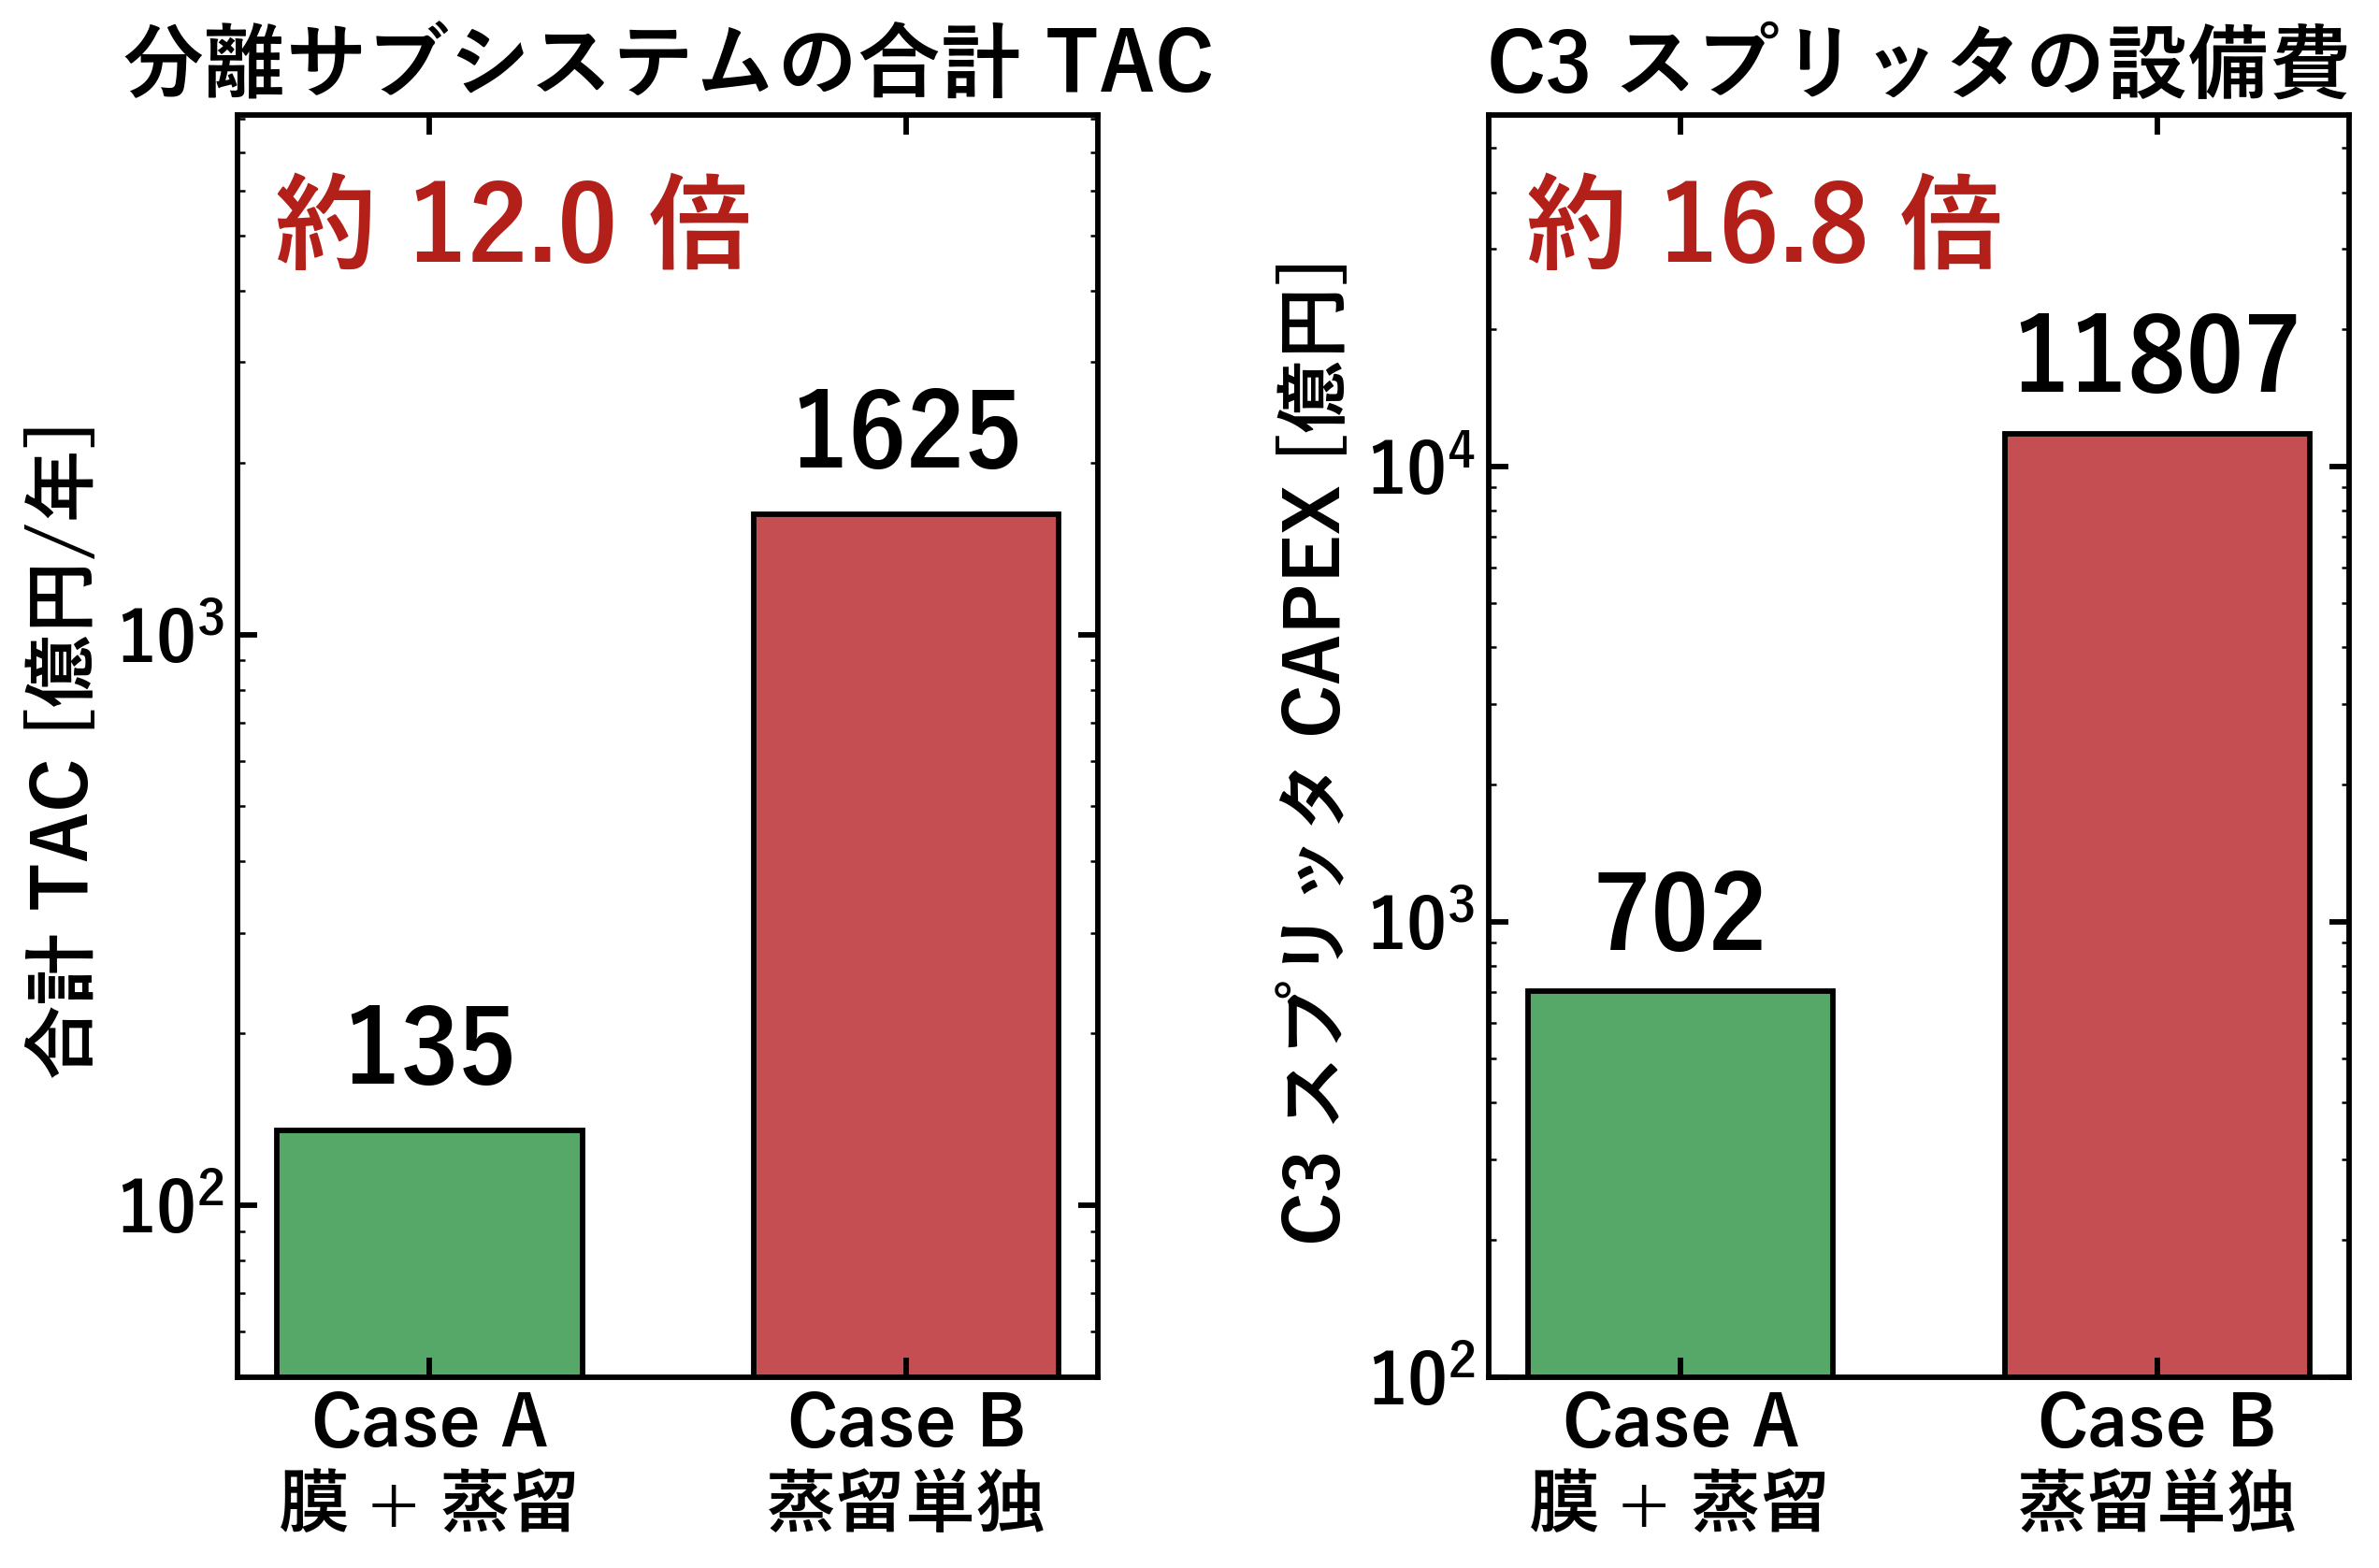
\includegraphics[width=\linewidth]{membrane_vs_dist3_slide}\par
      \vspace{0.08em}
      \raggedright
      {\scriptsize 膜無しは塔単独で $200$ 段・塔高 $156$ m を要する。}
    \end{column}
  \end{columns}

\end{frame}

\section{蒸留分離}% =====================================================================
%  11  蒸留塔設計 — 左上=諸元表／右上=実寸比タワー図／下は空ける
%  source_memo: 05/06/07章＋trial #201。脱ブタン C3H8/C4H10 36段33m P19.5 全凝縮 α大／
%   脱エタン C2H6/C3H8 61段52m P7.9 部分凝縮 α3.9／C3 C3H6/C3H8 117段94m P16.7 全凝縮 α1.07(最難)。
%  方針：タイトル・共通設計枠組み・モデル名(SM/HYSYS)は載せない。表(左上)＋実寸比タワー(右上)。
%   下半分は意図的に空ける(後で別要素)。色は最難C3の赤のみ。丸括弧禁止。
% =====================================================================
\begin{frame}[t]

  \vspace{-0.7em}

  \begin{columns}[T,onlytextwidth]
    % ===== 左上：諸元表（SM/HYSYS は載せない／塔高は図側）=========
    \begin{column}{0.64\textwidth}
      {\scriptsize
       \setlength{\tabcolsep}{3pt}\renewcommand{\arraystretch}{1.04}%
       \begin{tabular}{@{}l c c c@{}}
         \toprule
          & 脱ブタン塔 & 脱エタン塔 & {\color{SpRed}C3 スプリッタ} \\
         \midrule
         軽／重キー & $\mathrm{C_3H_8}/\mathrm{C_4H_{10}}$ & $\mathrm{C_2H_6}/\mathrm{C_3H_8}$ & {\color{SpRed}$\mathrm{C_3H_6}/\mathrm{C_3H_8}$} \\
         塔頂留分 & $\mathrm{C_3H_8}$ & \begin{tabular}[t]{@{}c@{}}$\mathrm{H_2}\!\cdot\!\mathrm{CH_4}$\\[1pt]$\mathrm{C_2H_4}\!\cdot\!\mathrm{C_2H_6}$\end{tabular} & {\color{SpRed}$\mathrm{C_3H_6}$} \\
         比揮発度 $\alpha$ & 大 & $\approx 3.9$ & {\color{SpRed}\boldmath$\approx 1.07$} \\
         操作圧力 [bar] & $19.5$ & $7.9$ & {\color{SpRed}$16.7$} \\
         理論段数 & $36$ & $61$ & {\color{SpRed}\boldmath$117$} \\
         塔径 [m] & $4.0$ & $5.9$ & {\color{SpRed}$7.4$} \\
         還流比 & $2.0$ & $11.8$ & {\color{SpRed}$12.0$} \\
         フィード段 & $28$ & $31$ & {\color{SpRed}$96$} \\
         凝縮器 & 全凝縮 & 部分凝縮 & {\color{SpRed}全凝縮} \\
         リボイラ [MW] & $15.6$ & $44.2$ & {\color{SpRed}\boldmath$60.8$} \\
         \bottomrule
       \end{tabular}}
    \end{column}

    % ===== 右上：実寸比タワー図（名前＋塔高のみ）=================
    \begin{column}{0.36\textwidth}
      \centering
      \begin{tikzpicture}[
        x=1cm, y=1cm, >=Stealth, font=\scriptsize,
        name/.style={align=center, font=\scriptsize\bfseries},
        nameR/.style={align=center, font=\scriptsize\bfseries, text=SpRed},
      ]
        % 幅は塔径 D[m] に比例（4.0/5.9/7.4）、高さは塔高に比例（33/52/94m）
        % 脱ブタン D4.0 H33m
        \def\hB{1.34}\def\cB{0.55}\def\wB{0.33}
        \fill[pattern=horizontal lines, pattern color=HeaderBlue!55] (\cB-\wB,0) rectangle (\cB+\wB,\hB);
        \draw[HeaderBlue, line width=1pt] (\cB-\wB,0) rectangle (\cB+\wB,\hB);
        \node[name, anchor=south] at (\cB,\hB+0.06) {脱ブタン\\$33$ m};
        % 脱エタン D5.9 H52m
        \def\hE{2.11}\def\cE{1.9}\def\wE{0.49}
        \fill[pattern=horizontal lines, pattern color=HeaderBlue!55] (\cE-\wE,0) rectangle (\cE+\wE,\hE);
        \draw[HeaderBlue, line width=1pt] (\cE-\wE,0) rectangle (\cE+\wE,\hE);
        \node[name, anchor=south] at (\cE,\hE+0.06) {脱エタン\\$52$ m};
        % C3 D7.4 H94m（最難・赤）
        \def\hC{3.81}\def\cC{3.25}\def\wC{0.61}
        \fill[pattern=horizontal lines, pattern color=SpRed!50] (\cC-\wC,0) rectangle (\cC+\wC,\hC);
        \draw[SpRed, line width=1.2pt] (\cC-\wC,0) rectangle (\cC+\wC,\hC);
        \node[nameR, anchor=south] at (\cC,\hC+0.06) {C3 スプリッタ\\$94$ m};
        % 基準線＋注記
        \draw[black!35, line width=0.5pt] (\cB-0.5,0) -- (\cC+\wC+0.2,0);
      \end{tikzpicture}
    \end{column}
  \end{columns}

  \vspace{0.1em}

  % ===== 下：3塔の段プロファイル（組成・温度）全幅 =====
  \centering
  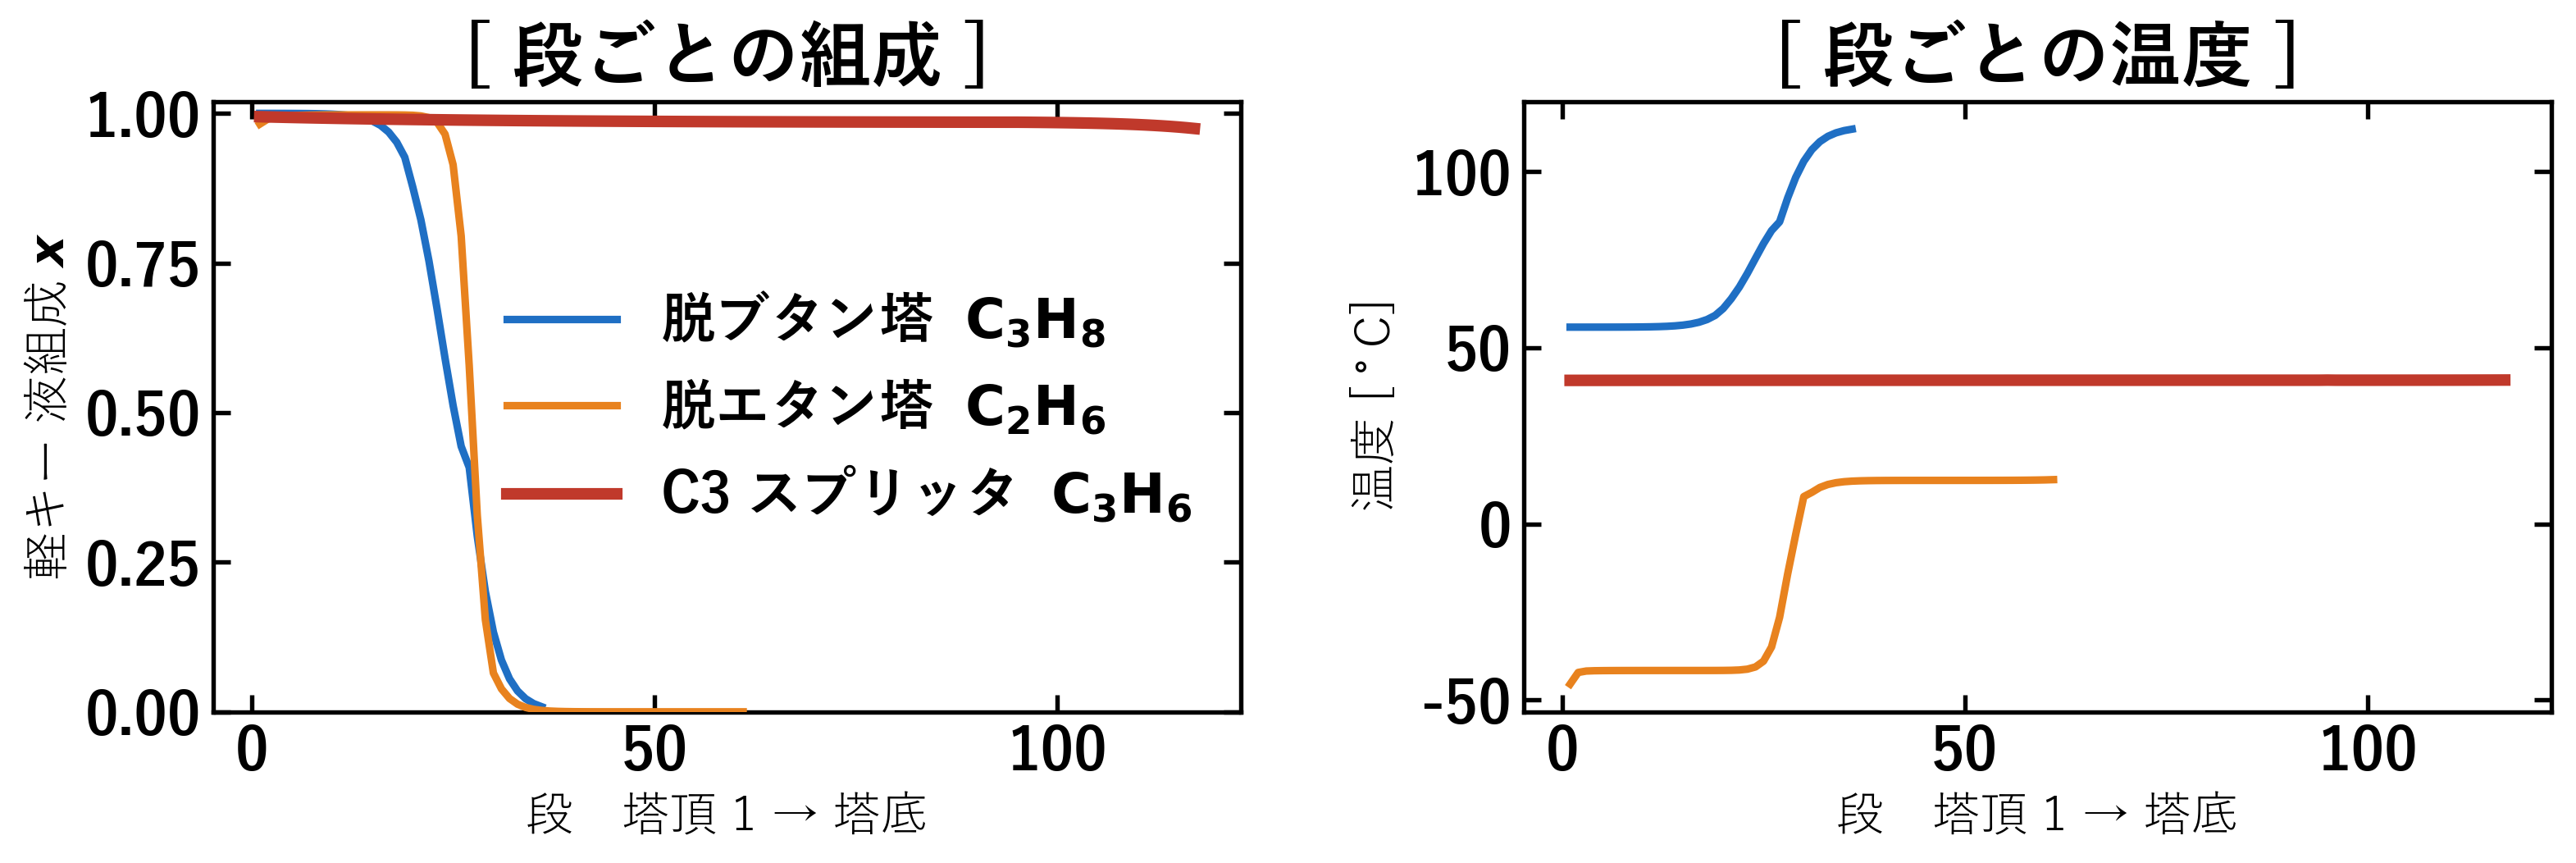
\includegraphics[width=0.97\linewidth]{dist_profiles}\par
  \vspace{0.12em}
  {\footnotesize\raggedright
   {\color{ArrowBlue}\textbf{脱ブタン}}・{\color{DipeOrange}\textbf{脱エタン}}：少ない段で組成・温度が急変化 ＝ 沸点差が大きく分離容易\par
   {\color{SpRed}\textbf{C3 スプリッタ}}：$117$ 段でも組成・温度ほぼ一定 ＝ 沸点差 $6$ K・$\alpha\!\approx\!1.07$ で分離困難\par}

\end{frame}

\section{膜分離}% =====================================================================
%  12  プロピレン精製 — 膜ユニット（2段：上=概念図/プロファイル、下=表/膜選定）
%  source_memo: 07章＋top1_trial201.txt[Membrane]＋Hua et al. ACS AMI 2024,16,15273.
%   ZIF-8細孔4.0-4.2Å。多結晶ZIF-8膜 SF~300/52GPU(大面積化・高コスト難)。ポリマー膜=トレードオフ・可塑化。
%   ZIF-8 混合マトリックス膜(添加剤併用in-situ形成): 無添加57.7/22.5・最高222.5/10.1・頑健量産版74.9/26.6GPU。採用α90/40=楽観側。
%  方針：図で一目＋口頭。膜=緑SepGreen。丸括弧禁止。余白を作らず最下部まで使う。
% =====================================================================
\definecolor{SepGreen}{HTML}{2E9E5B}
\definecolor{DipeOrange}{HTML}{E8821E}
\begin{frame}[t]

  \vspace{0.1em}

  % ===== 上段：膜分離器の概念図（左）／膜面積プロファイル（右）=====
  \begin{columns}[T,onlytextwidth]
    \begin{column}{0.45\textwidth}
      \raggedright
      {\footnotesize\bfseries\color{SepGreen!45!black} 膜分離器}\par
      \vspace{0.4em}
      \resizebox{\linewidth}{!}{%
      \begin{tikzpicture}[
        x=1cm, y=1cm, >=Stealth, font=\Large,
        c6/.style={circle, fill=SepGreen, draw=black, line width=0.4pt, minimum size=4mm, inner sep=0},
        c8/.style={circle, fill=DipeOrange, draw=black, line width=0.4pt, minimum size=6mm, inner sep=0},
        io/.style={align=center, font=\Large},
        pass/.style={-{Stealth[length=2.2mm]}, SepGreen!70!black, line width=1.1pt},
      ]
        % 膜（細孔つき）
        \fill[SepGreen!28] (2.4,0.2) rectangle (2.9,3.6);
        \draw[SepGreen, line width=1pt] (2.4,0.2) rectangle (2.9,3.6);
        \foreach \y in {0.7,1.4,2.1,2.8,3.3}{\fill[white] (2.4,\y-0.11) rectangle (2.9,\y+0.11);}
        \node[SepGreen!45!black, font=\Large\bfseries, anchor=south] at (2.65,3.7) {ZIF-8 膜};
        % 供給側（左）の分子：C3H8(橙)は残る、C3H6(緑)は透過
        \node[c8] at (1.0,2.9){}; \node[c6] at (1.75,3.1){}; \node[c8] at (1.3,2.0){};
        \node[c6] at (2.0,1.7){}; \node[c8] at (1.05,1.05){}; \node[c6] at (1.8,0.8){};
        % C3H6 が細孔を透過
        \draw[pass] (2.1,2.5)--(3.45,2.5); \draw[pass] (2.2,1.7)--(3.45,1.7); \draw[pass] (2.1,0.85)--(3.45,0.85);
        \node[c6] at (3.65,2.5){}; \node[c6] at (3.75,1.7){}; \node[c6] at (3.6,0.85){};
        % 供給（左、P_H 併記で重なり回避）
        \node[io, anchor=east] (f) at (-0.05,3.0) {供給 $\mathrm{C_3H_6}/\mathrm{C_3H_8}$\\[1pt]{\normalsize\bfseries\color{HeaderBlue}$P_H$ 8.4 bar}};
        \draw[-{Stealth[length=2.6mm]}, HeaderBlue, line width=1.4pt] (f.east) -- (0.7,3.05);
        % 非透過（下へ・矢印の下にラベル）
        \draw[-{Stealth[length=2.6mm]}, DipeOrange!80!black, line width=1.3pt] (1.5,0.0) -- (1.5,-0.75);
        \node[io, anchor=north, text=DipeOrange!70!black] at (1.5,-0.85) {非透過 $\mathrm{C_3H_8}$ → 循環};
        % 透過（右、98.6% 大・P_L 併記）
        \draw[pass, line width=1.5pt] (4.0,1.7)--(4.9,1.7);
        \node[io, anchor=west, text=SepGreen!45!black] at (4.95,2.15) {透過 $\mathrm{C_3H_6}$};
        \node[io, anchor=west, font=\LARGE\bfseries, text=SepGreen!45!black] at (4.95,1.45) {98.6\%};
        \node[io, anchor=west, font=\normalsize\bfseries, text=HeaderBlue] at (4.95,0.78) {$P_L$ 1 atm};
      \end{tikzpicture}}
    \end{column}

    \begin{column}{0.55\textwidth}
      \centering
      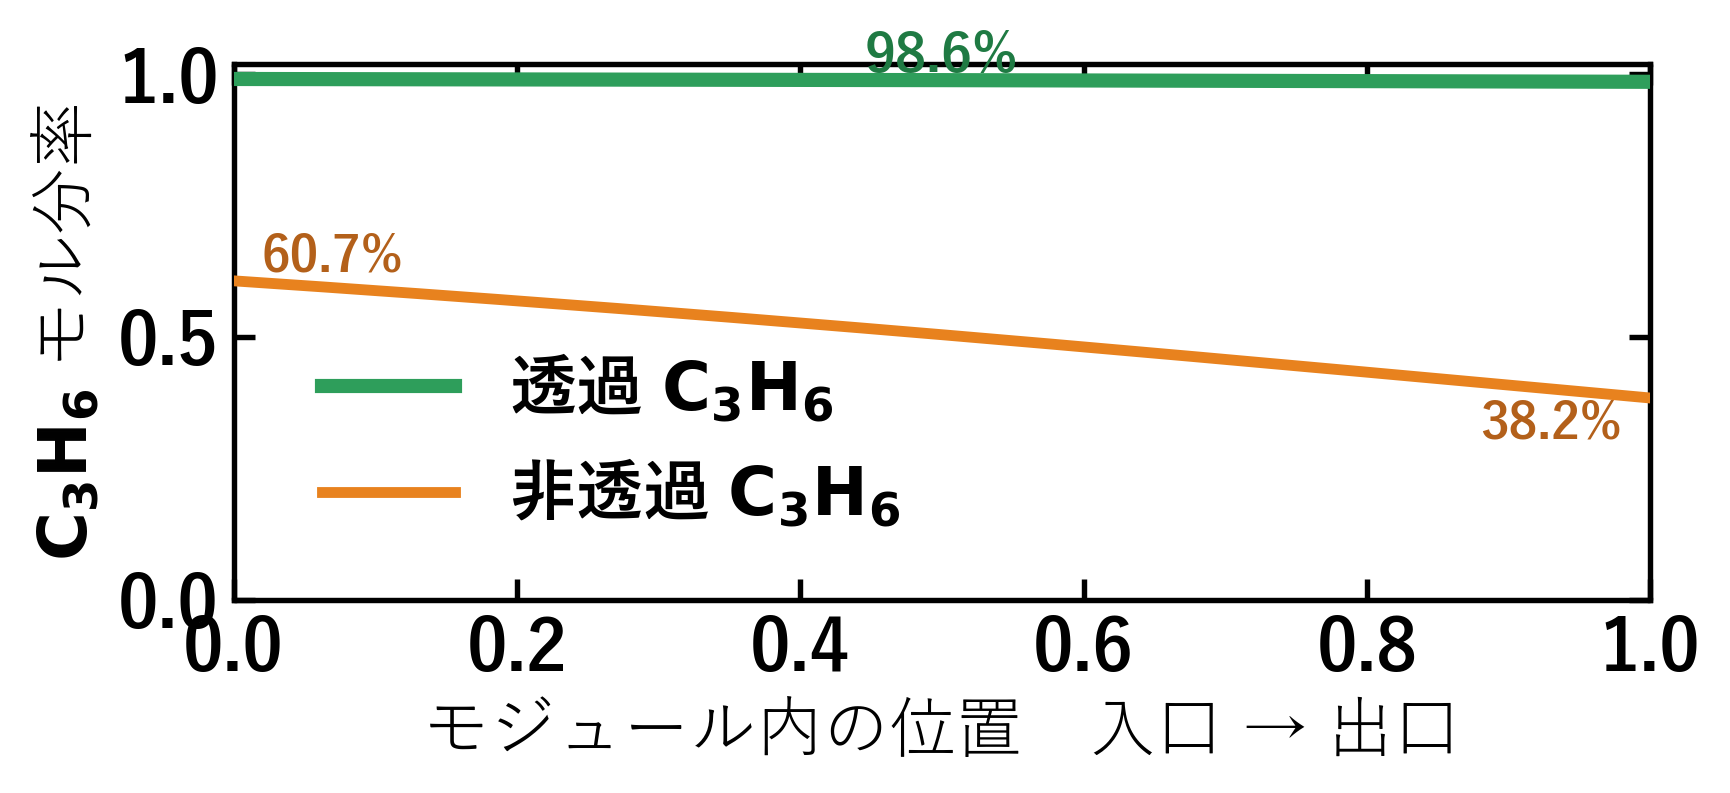
\includegraphics[width=\linewidth]{membrane_profile}\par
      \vspace{-0.82em}
      {\scriptsize モジュール内での $\mathrm{C_3H_6}$ 組成の変化}
    \end{column}
  \end{columns}

  \vspace{0.75em}

  % ===== 下段：設計変数表（左）／膜の選定 枠囲み（右）==========
  \begin{columns}[T,onlytextwidth]
    \begin{column}{0.37\textwidth}
      {\scriptsize\bfseries\color{HeaderBlue} 設計変数と性能}\par
      \vspace{0.12em}
      {\scriptsize\setlength{\tabcolsep}{5pt}\renewcommand{\arraystretch}{0.95}%
       \begin{tabular}{@{}l r@{}}
         \toprule
         供給圧 $P_H$ & $8.4$ bar \\
         膜面積 $A_{\mathrm{mem}}$ & $1.28\times10^{5}$ m$^2$ \\
         \midrule
         選択性 $\alpha$ & $90$ \\
         透過度 $Q_A$ & $40$ GPU \\
         透過圧 $P_L$ & $1$ atm \\
         \midrule
         モジュール数 & $256$ 本 \\
         ステージカット & $37$ \% \\
         透過純度 $\mathrm{C_3H_6}$ & $98.6$ mol\% \\
         \bottomrule
       \end{tabular}}\par
      \vspace{0.12em}
      {\tiny\color{black!55} 上2行が最適化変数\par
       \vspace{0.10em}
       GPU：気体透過率の単位\par
       \smash{$1\,\mathrm{GPU}=3.35\times10^{-10}\ \mathrm{mol\,m^{-2}s^{-1}Pa^{-1}}$}\par
       \vspace{0.6em}
       {\color{black!50} 出典　Hua et al., ACS AMI, 16, 15273, 2024}}
    \end{column}

    \begin{column}{0.63\textwidth}
      {\setlength{\fboxsep}{6pt}\setlength{\fboxrule}{1.2pt}%
       \fcolorbox{SepGreen!55!black}{SepGreen!6}{%
        \begin{minipage}[t][4.0cm]{0.93\linewidth}
         {\scriptsize\bfseries\color{SepGreen!40!black} 膜の選定　ZIF-8 を高分子に分散した混合マトリックス膜}
         \vfill
         {\scriptsize\setlength{\tabcolsep}{4pt}\renewcommand{\arraystretch}{1.1}%
          \begin{tabular}{@{}l c c l@{}}
            \toprule
            膜種 & $\alpha$ & 透過 GPU & 特徴 \\
            \midrule
            多結晶 ZIF-8 & $\sim\!300$ & $52$ & 大面積化・高コスト \\
            高分子膜 & 低 & --- & 可塑化・低性能 \\
            {\bfseries\color{SepGreen!40!black} 採用 混合膜} & {\bfseries 90} & {\bfseries 40} & 量産可・高選択 \\
            \bottomrule
          \end{tabular}}
         \vfill
         {\scriptsize\raggedright 高選択の鍵\par \textbf{小さい非晶質 ZIF-8}・添加剤併用の in-situ 形成で量産\par}
         \vfill
         {\scriptsize\raggedright {\color{SpRed}\textbf{!}}\ 実験室レベル　大面積・連続化で低下＝採用値は楽観側\par}
         \vfill
         {\scriptsize\raggedright 実機の劣化要因：可塑化・競争吸着・濃度分極 等\par}
        \end{minipage}}}
    \end{column}
  \end{columns}

\end{frame}

\section{PSA}% =====================================================================
%  13  水素分離 — PSA（2段：上=概念図/吸着等温線、下=設計変数表/方式選定）
%  source_memo: 08章＋psa_system.py＋top1_trial201.txt[PSA]。活性炭・多成分Langmuir(Choi2003)
%   ＋LDF・1D PDE。H2非吸着で全量製品、CH4/C2H4/C2H6を吸着。破過基準0.1%。
%   最適化変数: 塔径D4.49m・層高L24.8m・脱着目標β0.254。導出 t_abs742/t_des113s・2基。
%   H2回収~84%・H2純度>99.9%・CH4捕捉100%。入1486(H2 60%)→H2製品746＋オフガス740 kmol/h。
%  方針：図で一目＋口頭。H2=緑、吸着成分=暖色。丸括弧禁止。余白を作らず最下部まで。
% =====================================================================
\definecolor{SepGreen}{HTML}{2E9E5B}
\definecolor{DipeOrange}{HTML}{E8821E}
\begin{frame}[t]

  \vspace{0.1em}

  % ===== 上段：PSA概念図（左）／吸着等温線（右）=================
  \begin{columns}[T,onlytextwidth]
    \begin{column}{0.46\textwidth}
      \raggedright
      {\footnotesize\bfseries\color{HeaderBlue} PSA　圧力スイング吸着}\par
      \vspace{0.3em}
      \centering
      \resizebox{\linewidth}{!}{%
      \begin{tikzpicture}[
        x=1cm, y=1cm, >=Stealth,
        bed/.style={draw, line width=1pt, minimum width=1.4cm, minimum height=2.1cm,
                    align=center, font=\Large\bfseries, rounded corners=2pt},
        io/.style={align=center, font=\Large},
        a/.style={-{Stealth[length=2.8mm]}, line width=1.4pt},
      ]
        \node[bed, draw=HeaderBlue, fill=HiBlue!45, text=HeaderBlue] (A) at (0,0) {吸着\\高圧};
        \node[bed, draw=black!45, fill=black!8, text=black!55] (B) at (2.9,0) {脱着\\低圧};
        % 供給（左→A）
        \node[io, anchor=east] (feed) at (-1.55,0) {供給 $\mathrm{H_2}$ リッチ\\{\normalsize $1486$ kmol/h ・$60$\%}};
        \draw[a, HeaderBlue] (feed.east) -- (A.west);
        % H2 製品（A→上）
        \node[io, anchor=south, text=SepGreen!45!black] (h2) at (0,1.5) {$\mathrm{H_2}$ 製品 $>99.9$\%\\{\normalsize $746$ kmol/h}};
        \draw[a, SepGreen!70!black] (A.north) -- (h2.south);
        % オフガス（B→下）
        \node[io, anchor=north, text=DipeOrange!75!black] (off) at (2.9,-1.45) {オフガス → 燃料\\{\normalsize $740$ kmol/h}};
        \draw[a, DipeOrange!80!black] (B.south) -- (off.north);
        % スイング
        \draw[{Stealth[length=2mm]}-{Stealth[length=2mm]}, line width=0.9pt, black!55]
              (A.east) -- node[above, font=\normalsize, text=black!60]{スイング}(B.west);
      \end{tikzpicture}}
    \end{column}

    \begin{column}{0.54\textwidth}
      \centering
      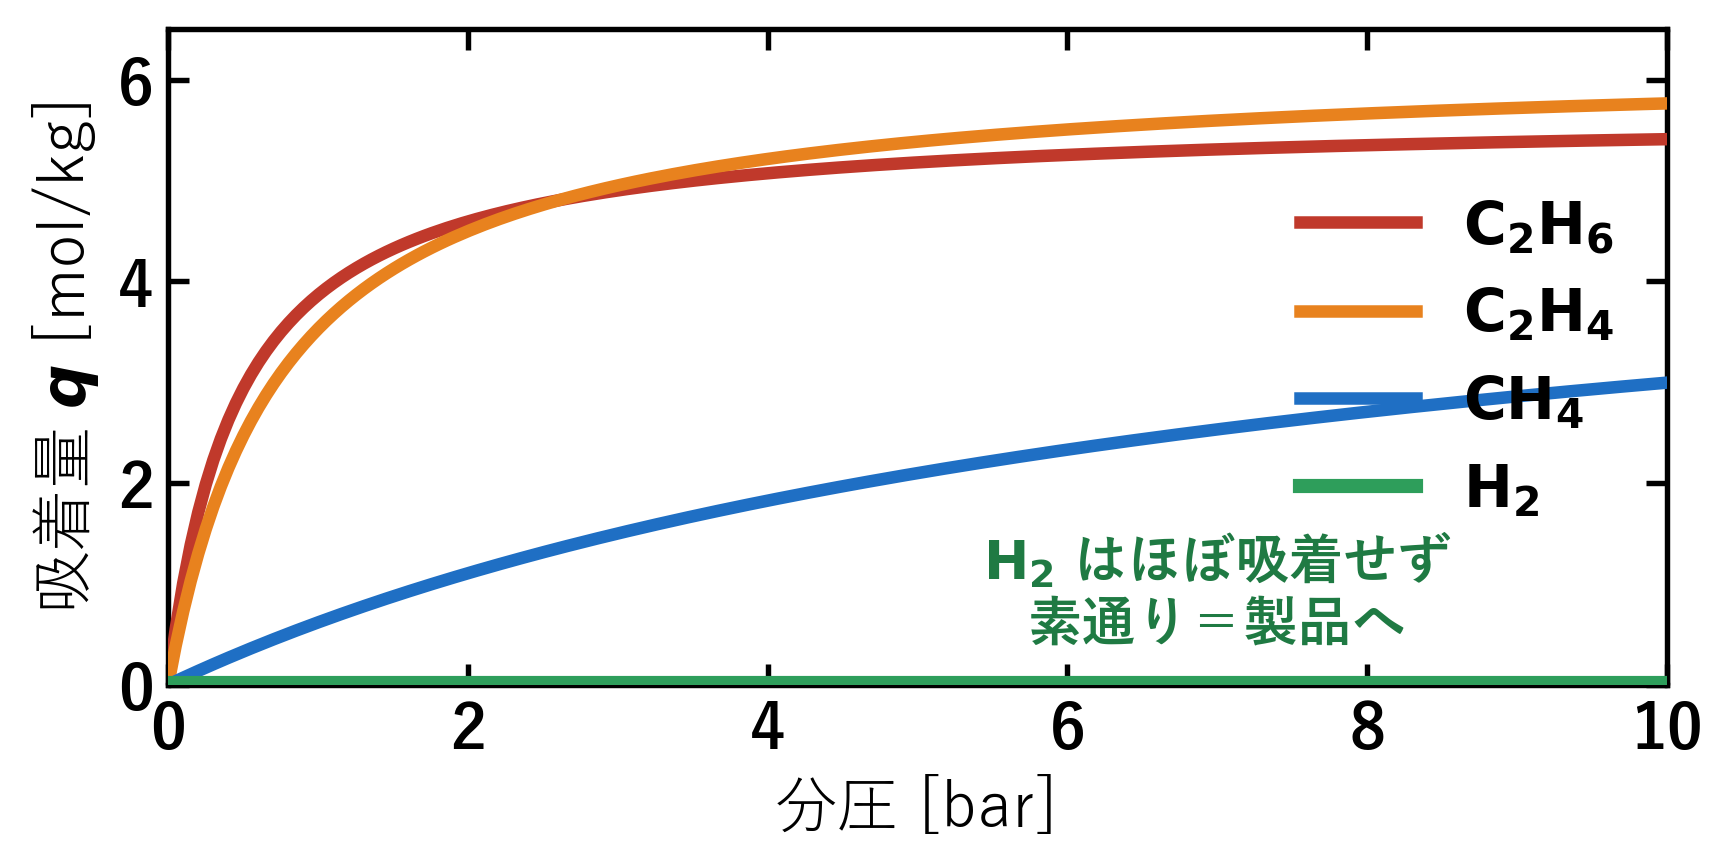
\includegraphics[width=\linewidth]{psa_isotherm}\par
      \vspace{-0.82em}
      {\scriptsize 活性炭の吸着等温線　$25\,^\circ$C}\par
      \vspace{0.12em}
      {\tiny\color{black!55} 出典：B.-U.\ Choi \textit{et al.}, J.\ Chem.\ Eng.\ Data, \textbf{48}(3), 603--607 (2003)}
    \end{column}
  \end{columns}

  \vspace{0.7em}

  % ===== 下段：設計変数表（左）／方式の選定 枠囲み（右）=========
  \begin{columns}[T,onlytextwidth]
    \begin{column}{0.37\textwidth}
      {\scriptsize\bfseries\color{HeaderBlue} 設計変数と諸元}\par
      \vspace{0.12em}
      {\scriptsize\setlength{\tabcolsep}{5pt}\renewcommand{\arraystretch}{1.02}%
       \begin{tabular}{@{}l r@{}}
         \toprule
         塔径 $D$ & $4.49$ m \\
         層高 $L$ & $24.8$ m \\
         脱着目標 $\beta$ & $0.254$ \\
         \midrule
         吸着材 & 活性炭 \\
         塔数 & $2$ 基 \\
         吸着／脱着時間 & $742$／$113$ s \\
         \midrule
         $\mathrm{H_2}$ 純度 & $99.9$\% 超 \\
         $\mathrm{H_2}$ 回収率 & 約 $84$\% \\
         $\mathrm{CH_4}$ 捕捉 & $100$\% \\
         \bottomrule
       \end{tabular}}\par
      \vspace{0.12em}
      {\tiny\color{black!55} 上3行が最適化変数}
    \end{column}

    \begin{column}{0.63\textwidth}
      {\setlength{\fboxsep}{6pt}\setlength{\fboxrule}{1.2pt}%
       \fcolorbox{HeaderBlue!70!black}{HiBlue!12}{%
        \begin{minipage}[t][4.13cm]{0.93\linewidth}
         {\scriptsize\bfseries\color{HeaderBlue} 方式の選定　PSA 圧力スイング吸着}
         \vfill
         {\scriptsize\setlength{\tabcolsep}{4pt}\renewcommand{\arraystretch}{1.1}%
          \begin{tabular}{@{}l c l@{}}
            \toprule
            方式 & $\mathrm{H_2}$ 純度 & 課題 \\
            \midrule
            深冷分離 & 高 & $-170\,^\circ$C 級・高コスト \\
            膜 & 中 & 高純度に多段が必要 \\
            {\bfseries\color{HeaderBlue} 採用 PSA} & {\bfseries $>99.9$\%} & 工業実績・連続 2 基 \\
            \bottomrule
          \end{tabular}}
         \vfill
         {\scriptsize\raggedright 吸着材＝\textbf{活性炭}：$\mathrm{H_2}$ 非吸着・$\mathrm{CH_4}/\mathrm{C_2}$ を選択吸着\par}
         \vfill
         {\scriptsize\raggedright 価値化：$\mathrm{H_2}$ は製品販売・\textbf{オフガスは予熱炉の燃料}\par}
        \end{minipage}}}
    \end{column}
  \end{columns}

\end{frame}

\end{document}
